\chapter{Proposta de Ferramenta}

Nesta seção, será apresentada uma ferramenta cujo objetivo é automatizar a geração de questões, com o objetivo de tornar mais fácil a construção e geração de questões. O sistema baseia-se em um modelo de separação entre duas entidades principais : (i) um JSON de template, responsável por definir a estrutura geral das questões; e (ii) um JSON de questões, que instancia as variações específicas de cada problema. 

\section{JSON de Template}
\begin{figure}[ht]
	\centering
	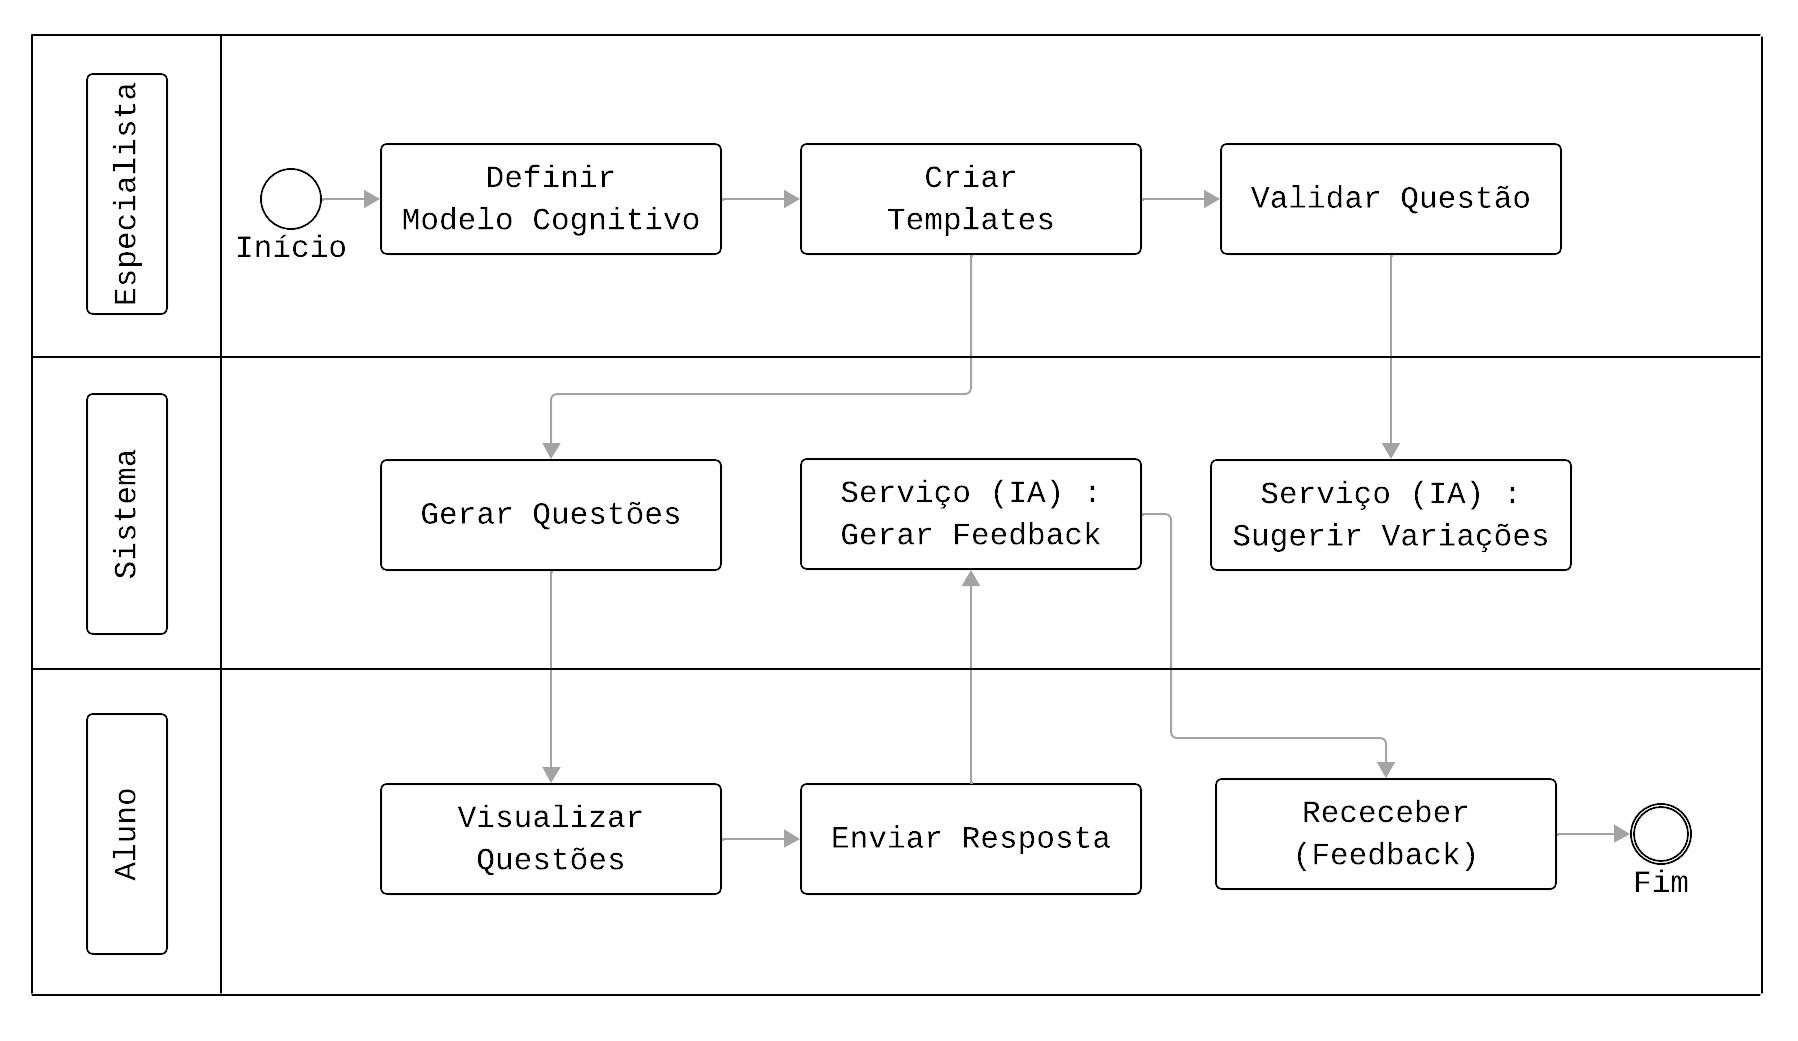
\includegraphics[width=14cm]{./imagens/capitulo6/bpmn-fluxo}
	\caption{BPMN do Fluxo de Trabalho (Autoria Propria, 2025) }
	\label{fig:bpmn-fluxo}
\end{figure}\begin{figure}
    \centering
    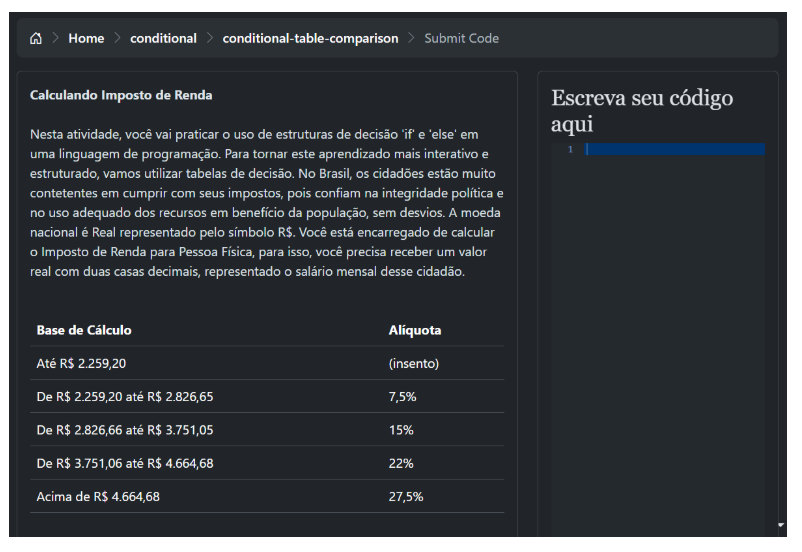
\includegraphics[width=0.5\linewidth]{imagens//capitulo7/repositorio-com-aig.png}
    \caption{Enter Caption}
    \label{fig:enter-label}
\end{figure}
\section{JSON de Questões}


\section{Ferramenta}